\chapter{Interfacing with LLDB}

We developed the first prototype of a native debugger for OCaml, based on the LLDB debugging framework on top of LLVM. For that, we first generated a full OCaml binding for the LLDB library, by parsing the C++ headers of the libraries and automatically generating OCaml and C++ stubs. We were then able to use the OCaml binding to develop several tools, ranging from a simple tool that displays the internal GC information of a finished OCaml application, to an almost complete debugger, which displays OCaml values using runtime type information added for memory profiling.

\section{Sub-component A\label{sec:conceptsuba}}
The concept chapter provides a high-level explanation of your solution. Try to explain the overall structure with a picture. You can also use UML sequence diagrams for explanation.

Figure \ref{fig:aliceandbob} illustrates the situation between Alice and Bob. (sequence diagram from www.websequencediagrams.com)

\begin{figure}[htb]
  \centering
  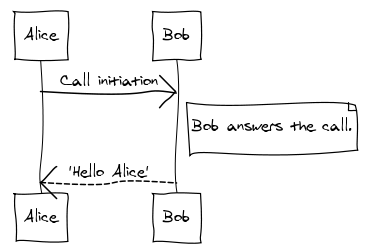
\includegraphics[width=9cm]{uml_seq_example.png}\\
  \caption{Alice and Bob}
  \label{fig:aliceandbob}
\end{figure}

\section{Sub-component B\label{sec:conceptsubb}}

Lorem Ipsum...

\section{Proposed API\label{sec:conceptsubb}}

Lorem Ipsum...

\section{Layer X\label{sec:conceptlayerx}}

Lorem Ipsum...

\section{Interworking of X and Y\label{sec:conceptinter}}

Lorem Ipsum...

\section{Interface Specification\label{sec:intspec}}

Lorem Ipsum...

